\input{preamble.tex}
\newcommand{\vect}[2]{(#1_1,\ldots, #1_#2)}
%%%%%%% nesting newcommands $$$$$$$$$$$$$$$$$$$
\newcommand{\function}[1]{\newcommand{\nvec}[2]{#1(##1_1,\ldots, ##1_##2)}}

\newcommand{\linode}[2]{#1_n(x)#2^{(n)}+#1_{n-1}(x)#2^{(n-1)}+\cdots +#1_0(x)#2=g(x)}

\newcommand{\vecoffun}[3]{#1_0(#2),\ldots ,#1_#3(#2)}

\newcommand{\suma}{\sum_{n=0}^{\infty}a_n x^n}

\newcommand{\sumb}{\sum_{n=1}^{\infty}a_n n x^{n-1}}

\newcommand{\sumc}{\sum_{n=2}^{\infty}a_n n (n-1) x^{n-2}}

\newcommand{\varsum}[2]{\sum_{n=#1}^{#2}}
\input{tikz.tex}



\begin{document}

\begin{tikzpicture}
  \draw[-latex,thick] (0,0) -- (3,0) node[right] {x};
  \draw[-latex,thick] (0,0) -- (0,3) node[above] {y};
  \draw (0,2) node[label=left:{$(0,b-a \lambda)$}] (a) {} -- 
    node[above right,midway] (p) {$ P(a,b)$} 
    (2.4,0) node[label=below:{$(a-b/ \lambda, 0)$}] (b) {};
  \fill (0,2) circle[radius=1.5pt];
  \fill (2.4,0) circle[radius=1.5pt];
  \fill ($ (a)!.5!(b)$) circle[radius=1.5pt];
\end{tikzpicture}
\hfill 
\begin{tikzpicture}
  \node (0) at (-2, 0) {};
  \node (1) at (3, 0) {};
  \node (2) at (-1, 2) {};
  \node (3) at (-1, 0) {};

  \node at (0) [left] {$B$};
  \node at (1) [right] {$\Gamma$};
  \node at (2) [above] {$A$};
  \node at (3) [below] {$\Delta$};

  \draw (0.center) to (1.center);
  \draw[name=ab] (0.center) to (2.center);
  \draw[name path=ac] (2.center) to (1.center);
  \draw[dashed] (2.center) -- (3.center) node[midway,right] {$h$};

  \node at ($(0)!.65!(2)$) [left=3pt] {Z};
  \fill ($(0)!.65!(2)$) coordinate (z) circle[radius=1.5pt];
  \path[name path=zh] ($(0)!.65!(2)$) -- ([xshift=2pt]$(0)!.65!(2)$) coordinate (f);
  \draw (z) -- (intersection of z--f and 2--1) coordinate (h);
  \node at (h) [right=8pt] {$H$};
  \fill (h) circle[radius=1.5pt];
  \draw (z) |- (3);
  \draw (h) |- (3);
  \fill (z|-3) coordinate (r) circle[radius=1.5pt];
  \fill (h|-3) coordinate (k) circle[radius=1.5pt];
  \fill (2|-z) coordinate (e) circle[radius=1.5pt];
  \node at (e) [above right] {$E$};
  \path (h)--(h|-3) node[midway,left]{y};
  \path (z|-3)--(h|-3) node[pos=.65,below]{x};
  \tkzMarkRightAngle(2,3,1);
\end{tikzpicture}


\begin{tikzpicture}[shorten/.style={shorten >=#1pt,shorten <=#1pt}]
		\node (0) at (0, 2) {};
		\node (1) at (0, -2) {};
		\node (2) at (-3, 0) {};
		\node (3) at (3, 0) {};
		\node (6) at (-2, 0) {};
		\node (7) at (2, 0) {};

    \draw [bend right=90,thick] (6.center) edge [pos=.75] coordinate (l) (7.center);
    \fill (l) circle[radius=1.5pt];
		\draw [bend left=90,thick] (6.center) edge [pos=.75] coordinate (m) (7.center);
    \fill (m) circle[radius=1.5pt];
    \node at (m) [above right] {$M(x,y)$};
    \path [bend right=90] (7.center) edge [pos=.75] coordinate (k) (6.center);
    \fill (k) circle[radius=1.5pt];
		\path [bend left=90] (7.center) edge [pos=.75] coordinate (n) (6.center);
    \fill (n) circle[radius=1.5pt];
    \path (n) rectangle (m);
    \draw (n) rectangle (m);
    \path[name path=yy] (0.center) -- (1.center);
    \path[name path=xx] (2.center) -- (3.center);
    \draw (0.center) edge[latex-,thick] (1.center);
    \draw (2.center) edge[-latex,thick] (3.center);
    \path[name path=km] (k) -- (m);
    \path[name path=ml] (m) -- (l);

    \coordinate (o) (0,0);
    \coordinate[red,name intersections={of=km and yy,by=a}];
    \coordinate[red,name intersections={of=ml and xx,by=b}];
    \draw [decorate,shorten=0.5,decoration={brace,amplitude=3pt,raise=3pt}] (o) -- (a) 
      node[midway,left=6pt] {y} ; 
    \draw [decorate,decoration={brace,amplitude=3pt,raise=3pt}] (b) -- (o) 
      node[midway,below=6pt] {x} ; 
    \draw[fill,blue!20,draw=black] (0,0) rectangle (m);
    \node at (.7,.5) {$E_{1}$};
    
\end{tikzpicture}
\hfill
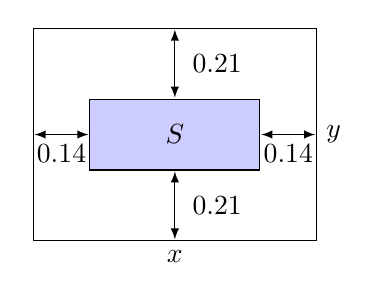
\begin{tikzpicture}[scale=0.9]
 \draw (0,0) rectangle (4,3);
 \draw[fill,blue!20] (.8,1) rectangle (3.2,2);
 \draw (.8,1) rectangle (3.2,2);

 \node at (2,1.5)  {$S$};
 \node at (2,0) [below] {$x$};
 \node at (4,1.5) [right] {$y$};
 \node (d) at (2,0.5) [right=.1cm] {\smaller$0.21$};
 \coordinate (dk) at (2,0) ;
 \coordinate (du) at (2,1) ;
 \node (p) at (2,2.5) [right=.1cm] {\smaller$0.21$};
 \coordinate (pk) at (2,2.0) ;
 \coordinate (pu) at (2,3) ;
 \draw (pk) edge[latex-latex,shorten >=0.5pt,shorten <=0.5pt,thin] (pu);
 \draw (dk) edge[latex-latex,shorten >=0.5pt,shorten <=0.5pt,thin] (du);
 \node (r) at (3.6,1.5) [below] {\smaller$0.14$};
 \coordinate (rl) at (3.2,1.5) ;
 \coordinate (rr) at (4,1.5) ;
 \draw (rl) edge[latex-latex,shorten >=0.5pt,shorten <=0.5pt,thin] (rr);
 \node (l) at (0.4,1.5) [below] {\smaller$0.14$};
 \coordinate (ll) at (0,1.5) ;
 \coordinate (lr) at (0.8,1.5) ;
 \draw (ll) edge[latex-latex,shorten >=0.5pt,shorten <=0.5pt,thin] (lr);
\end{tikzpicture}


\begin{tikzpicture}
  \draw (-2,0) -- (5,0);
  \coordinate (a') at (-1,0) ;
  \coordinate (e) at (1,0) ;
  \coordinate (b') at (4,0) ;
  \coordinate (a) at (-1,2) ;
  \coordinate (b) at (4,3) ;
  \node (x) at (0,0) [below] {$x$};
  \node (x') at (2.5,0) [below] {$20-x$};
  \node at (a') [below] {$A'$} ;
  \node at (b') [below] {$B'$} ;
  \node at (e) [below] {$E$} ;
  \draw (a') edge[-] node[midway,left] {10} (a);
  \draw (b') edge[-] node[midway,right] {15} (b);
  \draw (a) edge[dashed] (e);
  \draw (b) edge[dashed] (e);
  \node at (a) [above] {$A$} ;
  \node at (b) [above] {$B$} ;
\end{tikzpicture}
\end{document}
